\documentclass[11pt]{article}
\usepackage{graphicx}
\usepackage{amsmath}
\usepackage{pifont}
\usepackage{setspace}
\usepackage{hyperref}
\usepackage{enumitem}
\usepackage{color}
\usepackage{sectsty}
% \usepackage{raisebox}
% \usepackage{geometry}
% \usepackage{fancyhdr}
% \pagestyle{fancy}
% \lfoot{\emph{CV: Christopher Harman after discussion with Dr. S. Flockton}}
\definecolor{darkblue}{rgb}{0.,0.,0.7}
\sectionfont{\color{darkblue}}
\subsectionfont{\color{darkblue}}

\oddsidemargin  -0.25in
\evensidemargin 0.25in
\textwidth      7.0in
\headheight     0.0in
\topmargin      -0.8in
%\textheight=9.5in
\textheight=10.0in
\onehalfspacing

\begin{document}
\thispagestyle{empty}

\title{Clear Cut: Algorithm Design}
% \author{Christopher Harman}
\maketitle
\tableofcontents

\newpage



%%%%%%%%%%%%%%%%%%%%%%%%%%%%%%%%%%%%%%%%%%%%%%%%%%%%%%%%%%%%
%%%%%%%%%%%%%%%%%%%%%% INPUT DATA DESCRIPTION %%%%%%%%%%%%%%%%%%%%%%%
%%%%%%%%%%%%%%%%%%%%%%%%%%%%%%%%%%%%%%%%%%%%%%%%%%%%%%%%%%%%

\section{Input data}
The input data is an image of arbitrary size, $M \times N$, where $M$ is the horizontal dimension and $N$ is the vertical dimension of the image. Most images have three channels (RGB = ``Red-Green-Blue"), this means an array with three $M \times N$ arrays. Images with exif data are checked and modified so that the image is imported in the intended orientation, e.g. in case the image is a photo taken from a phone camera.



%%%%%%%%%%%%%%%%%%%%%%%%%%%%%%%%%%%%%%%%%%%%%%%%%%%%%%%%%%%%
%%%%%%%%%%%%%%%%%%%%%%% IMAGE SIZE REDUCTION %%%%%%%%%%%%%%%%%%%%%%%
%%%%%%%%%%%%%%%%%%%%%%%%%%%%%%%%%%%%%%%%%%%%%%%%%%%%%%%%%%%%

\subsection{Image size reduction}
To improve the efficiency of the edge detection algorithm, the image size is reduced to that the average image dimension is less than 500 pixels in length. The final image size to be thrown into the algorithm is $M_{\text{eff}} \times N_{\text{eff}}$, where
\begin{equation}
\dfrac{M_{\text{eff}} N_{\text{eff}}}{2}<500~\text{pxl} \text{.}
\label{im_reduction_condition}
\end{equation}
The image is currently reduced slowly by max pooling. This relies on calculating the smallest kernel size and repeating the max pooling process until the condition in Equation~\ref{im_reduction_condition} is satisfied. This can be implemented more effectively by calculating the smallest kernel that would satisfy the condition in Equation~\ref{im_reduction_condition} after just one implementation of max pooling.

As it currently exists, the process consists of determining the smallest number that divides the height (width) of the image to return an integer. If there is no such factor, i.e. the height (width) is a prime number, the image is cropped by removing the single pixel row (column) at the $M_{\text{eff}}^{th}$ ($N_{\text{eff}}^{th}$) index. By definition this would result in that image dimension being divisible by 2, which is then the number of pixels of the smallest kernel in that dimension. Throughout the image reduction process, the values ~{($M_{\text{eff}}$,~$N_{\text{eff}}$,~$M_{\text{kernel}}$,~$N_{\text{kernel}}$)} are stored in a Python dictionary to keep a record of the image reduction history.



%%%%%%%%%%%%%%%%%%%%%%%%%%%%%%%%%%%%%%%%%%%%%%%%%%%%%%%%%%%%
%%%%%%%%%%%%%%%%%%%%% EDGE DETECTION PROCEDURE %%%%%%%%%%%%%%%%%%%%%
%%%%%%%%%%%%%%%%%%%%%%%%%%%%%%%%%%%%%%%%%%%%%%%%%%%%%%%%%%%%

\section{Edge detection procedure}
\subsection{\label{sec:grad_img}The gradient image}
\begin{center}
\texttt{For Python code, refer to the {\bf traceObjectsInImage()} function in edgeUtility.py}
\end{center}
In order to determine the edges of an image, we must choose a criteria to distinguishing a single pixel located at $(i_0,j_0)$ as being part of ``an edge''. We would refer to such pixels as ``edge pixels'' or ``non-edge pixels'' in future. This is achieved by mathematically comparing its value to those of its surrounding pixels. The simplest method to adopt is to consider only the pixels neighbouring pixels $(i,j)$, i.e. any combination of pixels that satisfy
\begin{equation}
i_0-1 \leq i \leq i_0+1\text{, and }j_0-1 \leq j \leq j_0+1\text{.}
\end{equation}
A more advanced technique could extend the range of neighbouring pixels. For a pixel not located on the perimeter of the image, it would have 8 neighbouring pixels.

The mathematical quantity we are interested in is the difference in value between a selected pixel and it's neighbouring pixels. For the simple case, an edge pixel would be identified as having a large difference in value between any adjacent neighbouring pixel and itself. This simplest case works well for an image with sharp edges, but not so well for an image with blurry edges. With eight neighbouring pixels, we would have to calculate eight gradients per pixel. It turns out that we can more efficient in calculating the gradients and only count four instead. This is because when the neighbouring pixel has the gradient calculated, it would be the same magnitude but a different sign. The sign is irrelevant for determining the ``sharpness'' between pixels. This means that the eight gradient per pixel method would double-count the number of gradients; therefore we need only calculate four gradients per pixel instead.

Thus for a generic pixel at $(i,j)$, the difference in value between pixels $(i-1,j-1)$, $(i+1,j)$, $(i,j+1)$, and $(i+1,j+1)$ is calculated. These four directions are a choice and are not expected to make a difference in the final result. Note that not all gradients can be calculated if the pixel under consideration sits along the perimeter of the image. That each pixel in the ``image space'' has four unique gradients calculated, means that we will obtain a ``gradient space'' of size $2M_{\text{eff}} \times 2N_{\text{eff}}$.

\subsection{Dealing with image channels}
\subsubsection{Obtaining gradient images}
\begin{center}
\texttt{For Python code, refer to the {\bf traceObjectsInImage()} function in edgeUtility.py}
\end{center}
Each of the RGB channels have the edge detection algorithm specified in Section~\ref{sec:grad_img} applied to them. This is achieved by writing out the results to a single array of size $6M_{\text{eff}} \times 2N_{\text{eff}}$, where each channel's gradient image is offset as follows:
\begin{itemize}
  \item the Red channel gradient array exists in the domain $(0,~2M_{\text{eff}}-1)$,
  \item the Green channel gradient array exists in the domain $(2M_{\text{eff}},~4M_{\text{eff}}-1)$, and
  \item the Blue channel gradient array exists in the domain $(4M_{\text{eff}},~6M_{\text{eff}}-1)$.
\end{itemize}
Recall that we could only reduce the number of gradients per pixel if we ignore the gradients sign. Therefore, we must take care to only add up the gradient images element-wise AFTER taking the magnitude of each element first. The initial step in edge detection is to determine whether an (rgb) pixel in the reduced image is, or is not, part of an edge; this turns each pixel into a ``yes'' or ``no'' (boolean) answer. We therefore set a numerical upper and lower limit on what is an edge pixel, and what is not. We implement this through a variable parameter called \texttt{imCut}, whereby an edge pixel is one in which the gradient lives between:
\begin{equation}
255\times \texttt{imCut}< \text{Gradient}_{\text{edge pixel}} < 255\times (1-\texttt{imCut})\text{.}
\end{equation}
We have found $\texttt{imCut} = 0.07 \pm 0.02$ to work effectively. We have found both the upper limit and lower limit are necessary to extract clear edge pixels for any image. The lower limit is understandable because it determines adjacent pixels with too similar a colour as not being an edge pixel, however, the upper limit is less trivial. We believe the upper limit is necessary to remove random fluctuations in light/darkness within an image. These may be the result of tiny defective regions of photographical film that cannot be seen by the human eye when the image view at a larger scale that the size of the defect.

\subsubsection{Returning detected edges in reduced image size}
\begin{center}
\texttt{For Python code, refer to the {\bf mergeChannelsTracedImage()} function in edgeUtility.py}
\end{center}
We now have three gradient space arrays. However, we only want one gradient space array to say whether a single (rgb) pixel in the reduced image is an edge or not. This means we that we need to merge each of the gradient arrays into a single gradient array, and then reduce this gradient array to be the same size as the reduced image. The idea behind the merge is that \textbf{the more channels that detect an edge, the more likely it is to be an edge}. This is in agreement with human perception that an orange boat on a blue sea is far more distinct object than a blue boat on a blue sea. We therefore simply add up each gradient image element-wise to form our final gradient image.

This final gradient image is still roughly double the width and double the height of the reduced image. We reduce the gradient image to the same size as the reduced image using max pooling of $(2 \times 2)$-sized kernels. Therefore the final ``edge value'' of each (rgb) pixel of the reduced image is determined by the largest gradient of that pixel and its neighbouring pixel. This in turn determines whether it is an edge pixel or not.

\subsection{Cleaning the edge data}
Now that we have two arrays of the same size, we can mask the edge image on top of the reduced image to view our current results. In doing so for a number of unique images, we observe  two main features:
\begin{enumerate}
  \item There exist spurious regions of edge pixels with a size of the order of a few pixels. \textbf{Solution: remove tiny regions of edge data.}
  \item There are edge pixels around the perimeter of objects in the reduced image, but with the occasional break, whereby no edge pixels exist. \textbf{Solution: extrapolate long regions of edge data.}
\end{enumerate}

\subsubsection{Removing small scale edge data}
\begin{center}
\texttt{For Python code, refer to the {\bf edgeKiller()} function in edgeUtility.py}
\end{center}
To accomplish this task, we first need to decide what a small scale is. This is necessary for object recognition because many complicated objects are made of smaller, perhaps even more complicated objects. Fundamentally, if an object is identified as being surrounded by a continuous border of edge pixels, then the smallest object would be three pixels in size. This because the border must be at least one pixel thick and the central pixel must not be recognised as an edge (two pixels either side of a non-edge pixel in the $x$ and $y$ direction), i.e. a square drawn around the perimeter of a $3 \times 3$ pixel grid. Practically, it is the choice of the user to specify a tolerance to the size of the object. Take the example of a cat. Users may want to extract certain features of the cat, depending on some objective scaling into the cat (see Table~\ref{cat_table}).

\begin{table}[h]
\begin{center}
\begin{tabular}{|c|c|c|c|c|c|}
\hline
{\bf Feature/object} & {\bf User 1} & {\bf User 2} & {\bf User 3} & {\bf User 4}\\
\hline
{\bf Cat} & y & y & y & y\\
\hline
{\bf Nose} & n & y & y & y\\
\hline
{\bf Eye} & n & n & y & y\\
\hline
{\bf Iris} & n & n & n & y\\
\hline
\end{tabular}
\end{center}
\label{cat_table}
\end{table}

To this end, a user may specific their pixel tolerance using the parameter \texttt{objectTolerance}. Any edge pixels that are found within a border of size $(2\times \texttt{objectTolerance}+1) \times (2\times \texttt{objectTolerance}+1)$, where the border does not contain any edge pixels, are killed off.

% include visualisations here

\subsubsection{Expand large-length edge data}
\begin{center}
\texttt{For Python code, refer to the {\bf edgeFiller()} function in edgeUtility.py}
\end{center}
To address the issue of small gaps within edges, we extrapolate any edges subject to number of consecutive edge pixels in a given direction. The minimum number of consecutive edge pixels required for the extrapolation to happen is embodied in the parameter \texttt{edge\_bias}. The extrapolation basically runs through each edge pixels and determines the number of consecutive edge pixels in each of the eight directions $(-1,-1)$, $(-1,0)$,$(-1,+1)$, $(0,-1)$, $(0,+1)$, $(+1,-1)$, $(+1,0)$,and $(+1,+1)$. If the number of edge pixels in a direction is greater than $\texttt{edge\_bias}$, change the first non-edge pixel in that direction to an edge pixel.

% include visualisations here

%%%%%%%%%%%%%%%%%%%%%%%%%%%%%%%%%%%%%%%%%%%%%%%%%%%%%%%%%%%%
%%%%%%%%%%%%%%%%%%%%% OBJECT EXTRACTION PROCEDURE %%%%%%%%%%%%%%%%%%%%%
%%%%%%%%%%%%%%%%%%%%%%%%%%%%%%%%%%%%%%%%%%%%%%%%%%%%%%%%%%%%

\section{Object extraction procedure}
\subsection{Theoretical set up}
Randomly pick an initial edge pixel. Determine the directions in which the neighbouring pixel is also an edge pixel. For the directions which have an edge pixel, (recursively) determine if the pixel in that same direction is also an edge pixel until it is not an edge pixel. Note down the number of edge pixels in this direction and add it to the number of edge pixels (until a non-edge pixel is found) in the exact opposite direction. This will result in four lengths - which we will call \textit{thicknesses} - in each of the directions:
\begin{itemize}
  \item horizontal: $(-1,0)\rightarrow (+1,0)$,
  \item vertical: $(0,-1)\rightarrow (0,+1)$, 
  \item positive gradient diagonal: $(-1,-1)\rightarrow (+1,+1)$, 
  \item negative gradient diagonal: $(-1,+1)\rightarrow (+1,-1)$.
\end{itemize}

The shortest thickness of consecutive edge pixels at the initial edge pixel will be referred to as the \textbf{race start line}. The length of the race start line is defined to be in the $\hat{y}$-direction of the Cartesian coordinate system $\hat{C}: (\hat{x},\hat{y})$. The initial direction of the \textbf{race path} must have a non-zero $\hat{x}$-component, i.e. the initial path vector is $\vec{O}=a\hat{x}+b\hat{y}$, where $a \neq 0$.

\subsection{Definition of an object}
\begin{center}
\texttt{We define an object within an image as the set of pixels that residue\\ within an enclosed path of edge pixels. The enclosed path must return\\ through the race start line with an $\hat{\texttt{x}}$-component that has the same sign\\ as that in
	 which the path was initialised.}
\end{center}
There are two very important concepts to understand within this definition:
\begin{itemize}
  \item \textit{... an enclosed path ...}: this means we should be able to draw a continuous path of edge pixels that start and end at the same edge pixel coordinate.
  \item \textit{... $\hat{x}$-component that has the same sign ...}: this means that the path of edge pixels must have an initial path vector with an $\hat{x}$-component with the same sign as the $\hat{x}$-component of the (final) path vector that crosses past the start race line. Since the path is determined by when the path has crossed the start race line, it means the path could not have gone back on itself whereby it remains along the ``same edge''. % Need to include visualisations here of starting at the bottom of a hangmans knot, and starting at the top of the knot.
\end{itemize}

\subsection{Stepping into the edge path}
The edge path cannot be stepped by an entirely random process as the code would take too long to run and possible return nonsense (see Brownian motion). However, neither can the steps be too systematic as this may guarantee that some forks in the edges are never taken, thus losing potential objects. At each step, there must be some notion of moving in a direction roughly orthogonal to the shortest pixel thickness that is also away from pixel at the previous step. Therefore, the step is chosen to be close to the vector orthogonal to the start line for that current pixel, but with a small random fluctuation in the ($\hat{y}$-)direction of the start line.

\begin{figure}[h!]
\centering
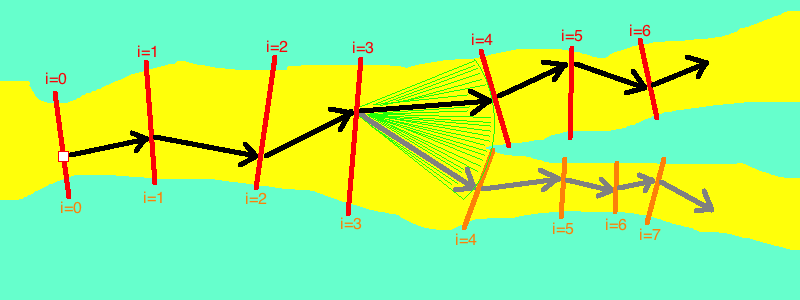
\includegraphics[width=15.0cm]{visuals/edge_id_aids/Path_algorithm.png}
\caption{\small{Visualisation of the random path method. This image shows two paths starting at the same initial edge pixel (white square) with the same steps up $i=3$. At this point the path the random vector off the $i=3$ start line may either go into the upper or lower fork of the edge. The green cone has been drawn to detail that the random path vector has a specified length (the radius of the cone) but the random direction is constrained to within the green cone.}}
\label{singleField_PtPlot_fig}
\end{figure}



\end{document}